\subsection*{Peano System Figure Plates}

\begin{exposition}
The following figure plates collect the visual diagrams for the Peano system
and iterator material. Each plate is presented separately so that the diagram
can be read as a full-page reference.
\end{exposition}

\begin{figure}[p]
\centering
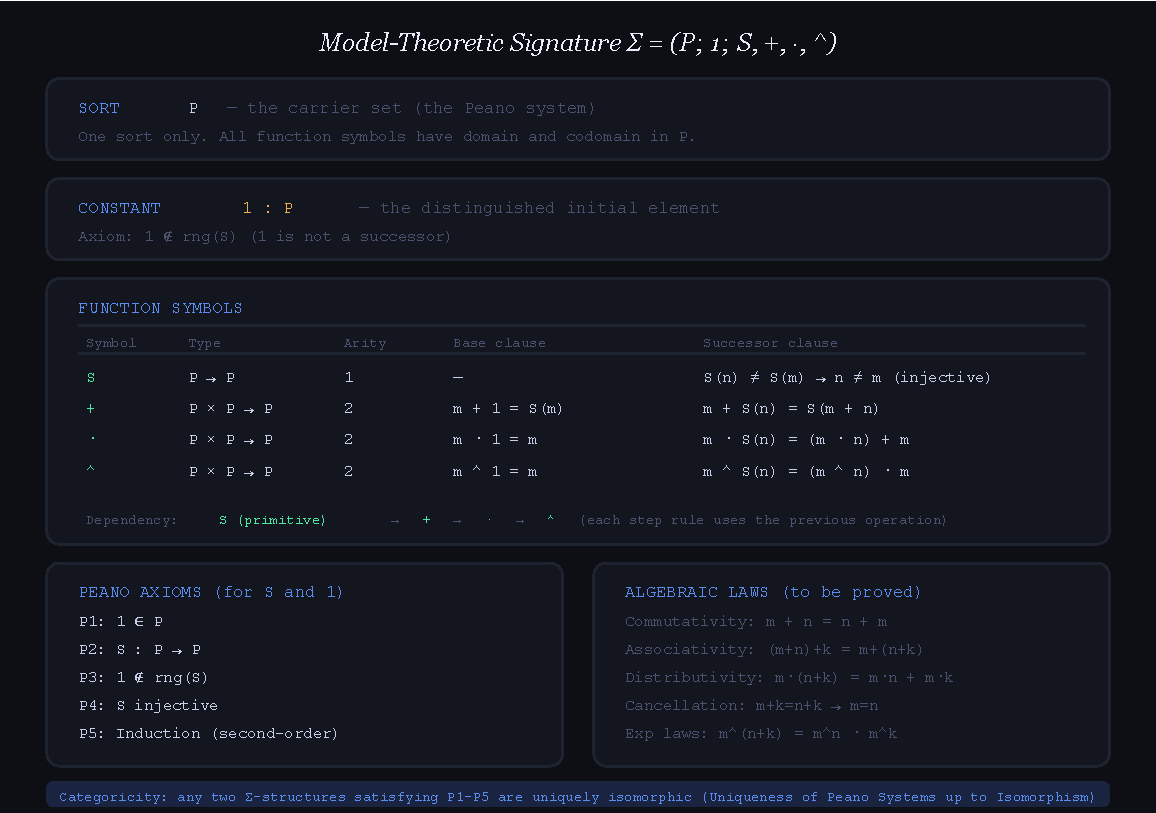
\includegraphics[width=\textwidth,height=0.78\textheight,keepaspectratio]
  {volume-ii/book-discrete-algebraic/peano-systems/notes/defining-peano-systems/diag_04_signature-asset.pdf}
\caption{The model-theoretic signature for a Peano system and the later
arithmetic operations generated from it.}
\end{figure}

\clearpage

\begin{figure}[p]
\centering
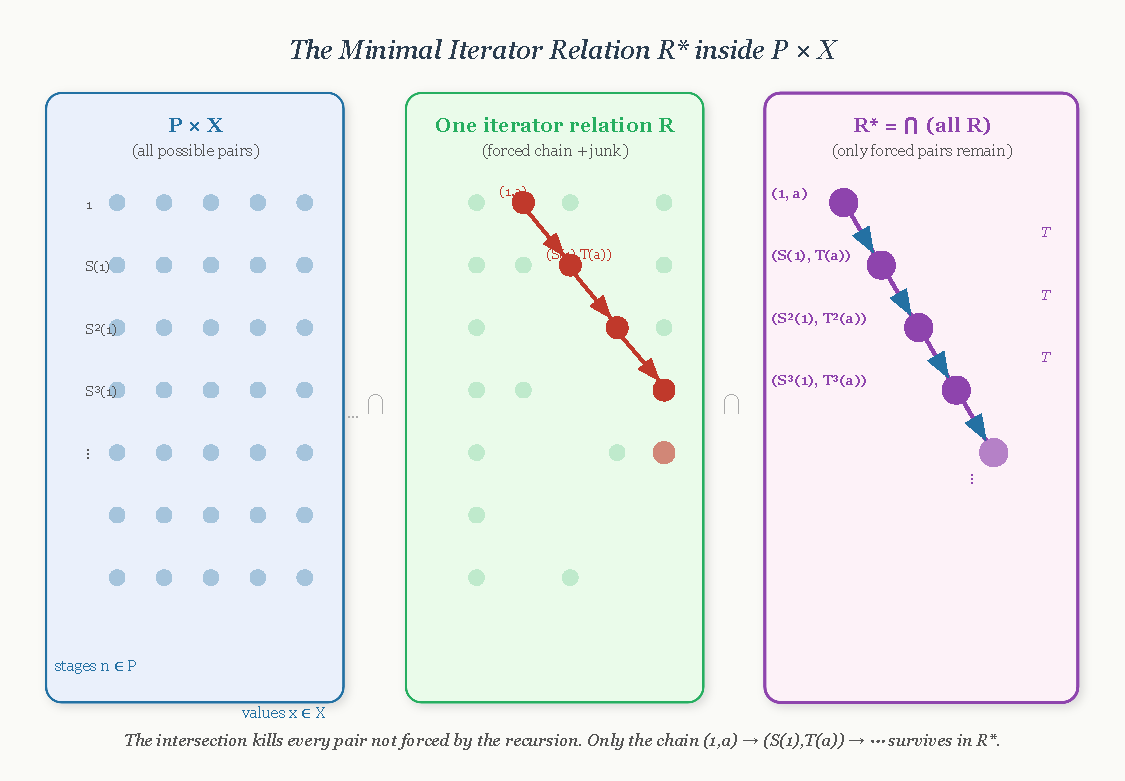
\includegraphics[width=\textwidth,height=0.78\textheight,keepaspectratio]
  {volume-ii/book-discrete-algebraic/peano-systems/notes/defining-peano-systems/diag_01_rstar_intuitive-asset.pdf}
\caption{The intuitive construction of the minimal iterator relation $R^*$
inside $P\times W$.}
\end{figure}

\clearpage

\begin{figure}[p]
\centering
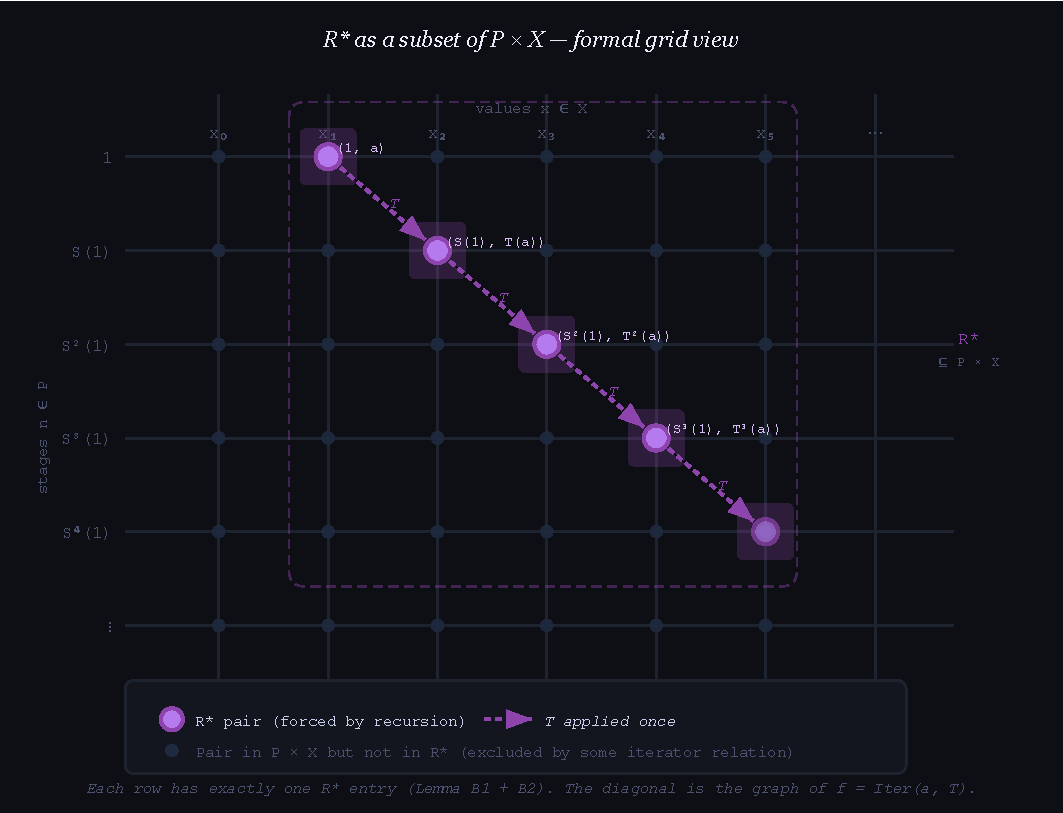
\includegraphics[width=\textwidth,height=0.78\textheight,keepaspectratio]
  {volume-ii/book-discrete-algebraic/peano-systems/notes/defining-peano-systems/diag_02_rstar_formal-asset.pdf}
\caption{A formal grid view of $R^*$ as the chain of forced ordered pairs in
$P\times W$.}
\end{figure}

\clearpage

\begin{figure}[p]
\centering
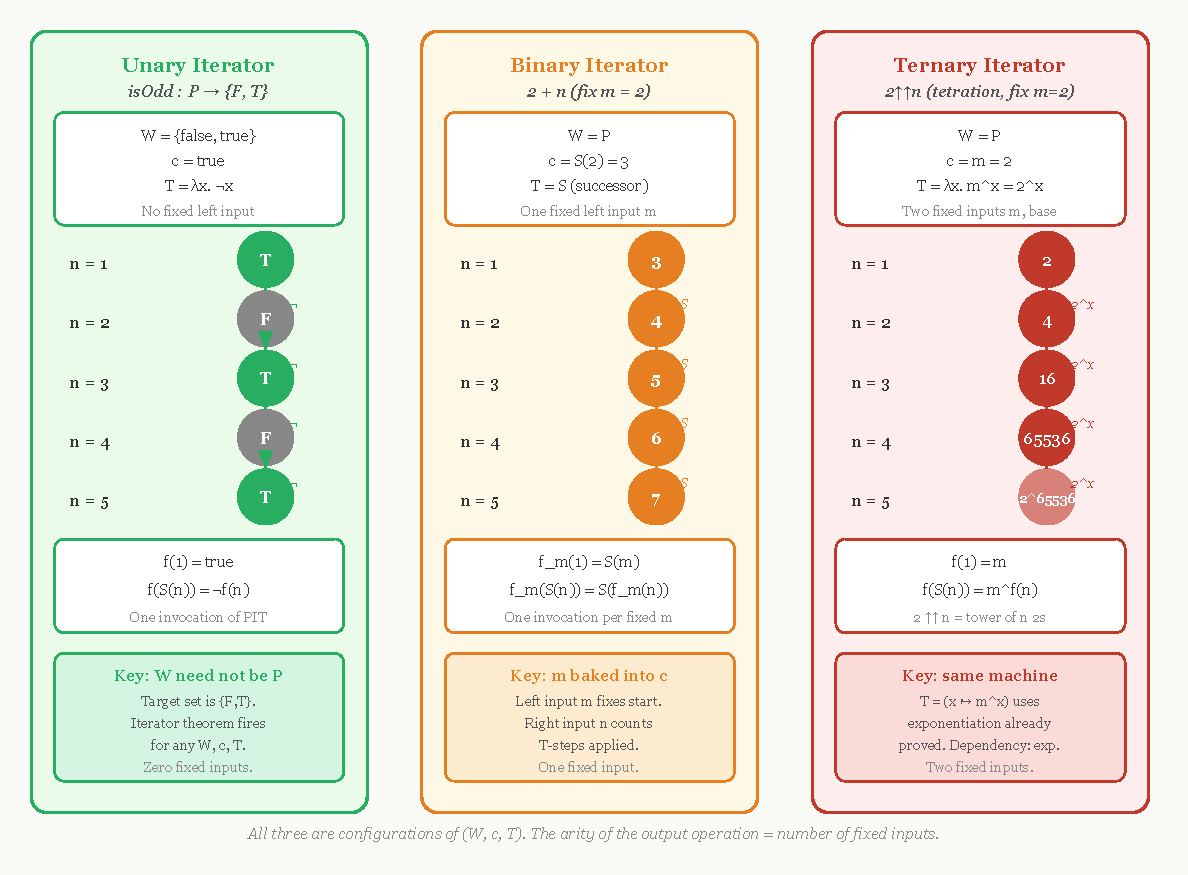
\includegraphics[width=\textwidth,height=0.78\textheight,keepaspectratio]
  {volume-ii/book-discrete-algebraic/peano-systems/notes/defining-peano-systems/diag_03_arity_examples-asset.pdf}
\caption{Unary, binary, and higher-arity iterator configurations after fixing
the relevant parameters.}
\end{figure}

\clearpage

\begin{figure}[p]
\centering
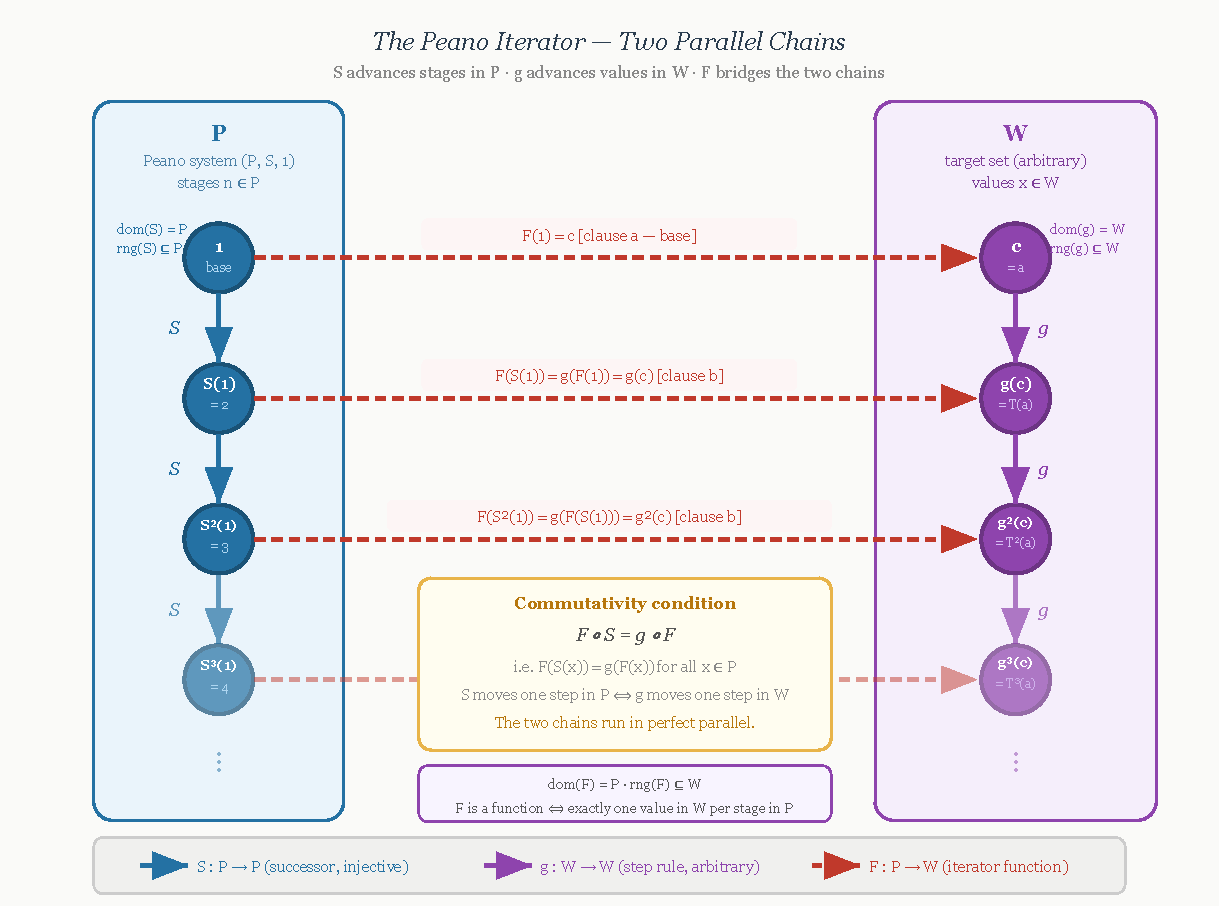
\includegraphics[width=\textwidth,height=0.78\textheight,keepaspectratio]
  {volume-ii/book-discrete-algebraic/peano-systems/notes/defining-peano-systems/diag_05_parallel_chains-asset.pdf}
\caption{The Peano iterator as two parallel chains, one in $P$ and one in
$W$, connected by the iterator function.}
\end{figure}

\clearpage

\begin{figure}[p]
\centering
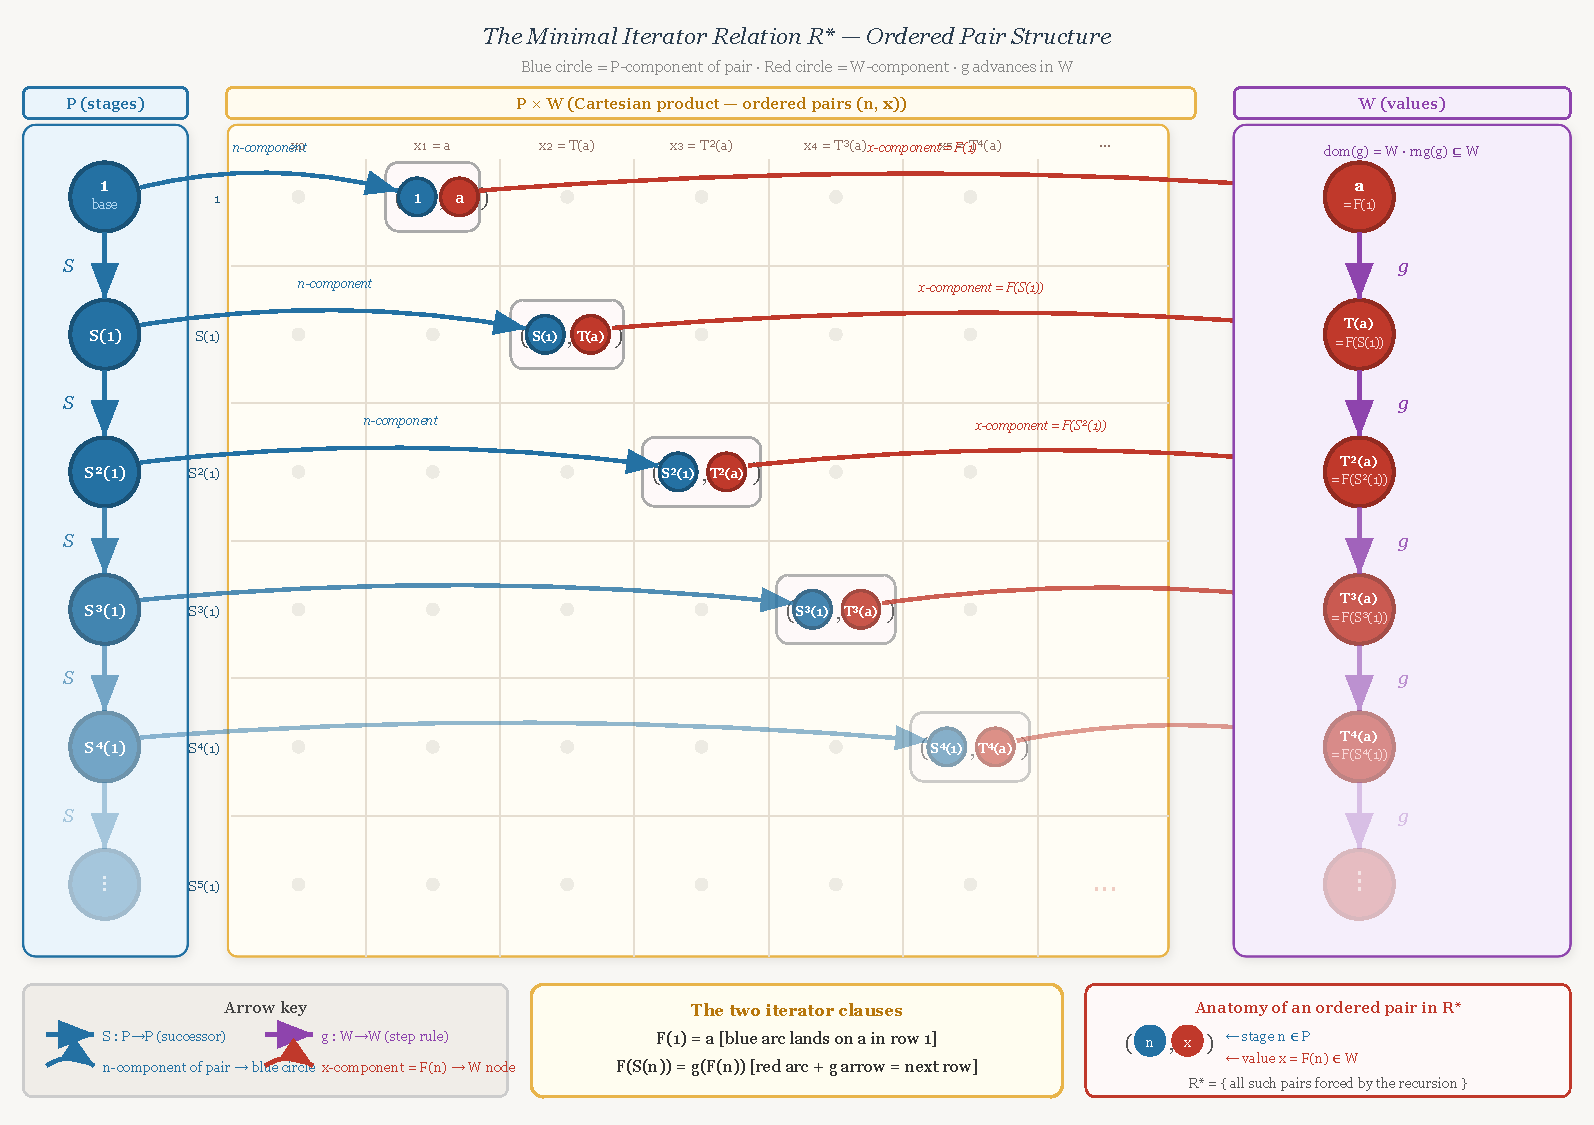
\includegraphics[width=\textwidth,height=0.78\textheight,keepaspectratio]
  {volume-ii/book-discrete-algebraic/peano-systems/notes/defining-peano-systems/diag_06_three_zone-asset.pdf}
\caption{The three-zone view of $R^*$, separating stages in $P$, ordered pairs
in $P\times W$, and values in $W$.}
\end{figure}

\clearpage
